\documentclass[journal, a4paper]{IEEEtran}

% some very useful LaTeX packages include:
\usepackage[brazil]{babel}
\usepackage[utf8x]{inputenc}
\usepackage{amsmath}
\usepackage{float}
\usepackage{mathtools}
\usepackage{natbib}
%\usepackage{multicol, blindtext}

%\usepackage{cite}      % Written by Donald Arseneau
                        % V1.6 and later of IEEEtran pre-defines the format
                        % of the cite.sty package \cite{} output to follow
                        % that of IEEE. Loading the cite package will
                        % result in citation numbers being automatically
                        % sorted and properly "ranged". i.e.,
                        % [1], [9], [2], [7], [5], [6]
                        % (without using cite.sty)
                        % will become:
                        % [1], [2], [5]--[7], [9] (using cite.sty)
                        % cite.sty's \cite will automatically add leading
                        % space, if needed. Use cite.sty's noadjust option
                        % (cite.sty V3.8 and later) if you want to turn this
                        % off. cite.sty is already installed on most LaTeX
                        % systems. The latest version can be obtained at:
                        % http://www.ctan.org/tex-archive/macros/latex/contrib/supported/cite/

\usepackage{graphicx}   % Written by David Carlisle and Sebastian Rahtz
                        % Required if you want graphics, photos, etc.
                        % graphicx.sty is already installed on most LaTeX
                        % systems. The latest version and documentation can
                        % be obtained at:
                        % http://www.ctan.org/tex-archive/macros/latex/required/graphics/
                        % Another good source of documentation is "Using
                        % Imported Graphics in LaTeX2e" by Keith Reckdahl
                        % which can be found as esplatex.ps and epslatex.pdf
                        % at: http://www.ctan.org/tex-archive/info/

\usepackage{psfrag}    % Written by Craig Barratt, Michael C. Grant,
                        % and David Carlisle
                        % This package allows you to substitute LaTeX
                        % commands for text in imported EPS graphic files.
                        % In this way, LaTeX symbols can be placed into
                        % graphics that have been generated by other
                        % applications. You must use latex->dvips->ps2pdf
                        % workflow (not direct pdf output from pdflatex) if
                        % you wish to use this capability because it works
                        % via some PostScript tricks. Alternatively, the
                        % graphics could be processed as separate files via
                        % psfrag and dvips, then converted to PDF for
                        % inclusion in the main file which uses pdflatex.
                        % Docs are in "The PSfrag System" by Michael C. Grant
                        % and David Carlisle. There is also some information
                        % about using psfrag in "Using Imported Graphics in
                        % LaTeX2e" by Keith Reckdahl which documents the
                        % graphicx package (see above). The psfrag package
                        % and documentation can be obtained at:
                        % http://www.ctan.org/tex-archive/macros/latex/contrib/supported/psfrag/

\usepackage{subfig} % Written by Steven Douglas Cochran
                        % This package makes it easy to put subfigures
                        % in your figures. i.e., "figure 1a and 1b"
                        % Docs are in "Using Imported Graphics in LaTeX2e"
                        % by Keith Reckdahl which also documents the graphicx
                        % package (see above). subfigure.sty is already
                        % installed on most LaTeX systems. The latest version
                        % and documentation can be obtained at:
                        % http://www.ctan.org/tex-archive/macros/latex/contrib/supported/subfigure/

\usepackage{url}        % Written by Donald Arseneau
                        % Provides better support for handling and breaking
                        % URLs. url.sty is already installed on most LaTeX
                        % systems. The latest version can be obtained at:
                        % http://www.ctan.org/tex-archive/macros/latex/contrib/other/misc/
                        % Read the url.sty source comments for usage information.

\usepackage{stfloats}  % Written by Sigitas Tolusis
                        % Gives LaTeX2e the ability to do double column
                        % floats at the bottom of the page as well as the top.
                        % (e.g., "\begin{figure*}[!b]" is not normally
                        % possible in LaTeX2e). This is an invasive package
                        % which rewrites many portions of the LaTeX2e output
                        % routines. It may not work with other packages that
                        % modify the LaTeX2e output routine and/or with other
                        % versions of LaTeX. The latest version and
                        % documentation can be obtained at:
                        % http://www.ctan.org/tex-archive/macros/latex/contrib/supported/sttools/
                        % Documentation is contained in the stfloats.sty
                        % comments as well as in the presfull.pdf file.
                        % Do not use the stfloats baselinefloat ability as
                        % IEEE does not allow \baselineskip to stretch.
                        % Authors submitting work to the IEEE should note
                        % that IEEE rarely uses double column equations and
                        % that authors should try to avoid such use.
                        % Do not be tempted to use the cuted.sty or
                        % midfloat.sty package (by the same author) as IEEE
                        % does not format its papers in such ways.

\usepackage{amsmath}    % From the American Mathematical Society
                        % A popular package that provides many helpful commands
                        % for dealing with mathematics. Note that the AMSmath
                        % package sets \interdisplaylinepenalty to 10000 thus
                        % preventing page breaks from occurring within multiline
                        % equations. Use:
\interdisplaylinepenalty=2500
                        % after loading amsmath to restore such page breaks
                        % as IEEEtran.cls normally does. amsmath.sty is already
                        % installed on most LaTeX systems. The latest version
                        % and documentation can be obtained at:
                        % http://www.ctan.org/tex-archive/macros/latex/required/amslatex/math/



% Other popular packages for formatting tables and equations include:

%\usepackage{array}
% Frank Mittelbach's and David Carlisle's array.sty which improves the
% LaTeX2e array and tabular environments to provide better appearances and
% additional user controls. array.sty is already installed on most systems.
% The latest version and documentation can be obtained at:
% http://www.ctan.org/tex-archive/macros/latex/required/tools/

% V1.6 of IEEEtran contains the IEEEeqnarray family of commands that can
% be used to generate multiline equations as well as matrices, tables, etc.

% Also of notable interest:
% Scott Pakin's eqparbox package for creating (automatically sized) equal
% width boxes. Available:
% http://www.ctan.org/tex-archive/macros/latex/contrib/supported/eqparbox/

% *** Do not adjust lengths that control margins, column widths, etc. ***
% *** Do not use packages that alter fonts (such as pslatex).         ***
% There should be no need to do such things with IEEEtran.cls V1.6 and later.


% Your document starts here!
\begin{document}

% Define document title and author
	\title{Relatório sobre o Mapa de Kohonen}
	\author{Victor Carreira
	\thanks{Professora: Marley. Eng. Elétrica. PUC-RIO}}
	\markboth{Trabalho 03}{}
	\maketitle

% Write abstract here
\begin{abstract}

\end{abstract}


\section{Introdução}
    As Redes Neurais Artificiais (RNA) são inspiradas em modelos sensoriais do processamento de tarefas realizadas pelo cérebro \citep{Hagan1996}. Uma RNA, portanto pode ser criada através da aplicação de algoritmos matemáticos que imitem a tarefa realizada por um neurônio \citep{Nedjah2016}. Uma rede neural artificial possui semelhanças com a rede biológica presente no sistema nervoso central, neste o cômputo de informações realizado do cérebro é feito através de uma vasta quantidade de neurônios interconectados \citep{Feldman1988,Poulton2002}. A comunicação entre essas células é realizada através de impulsos elétricos. Estes são transmitidos e recebidos por meio de sinapses nervosas entre axônios e dendritos. As sinapses são estruturas elementares e uma unidade funcional localizada entre dois neurônios \citep{Krogh2008}.

	%\citet{McCulloch1943} redigem o trabalho pioneiro onde foi modelado um neurônio cuja resposta dependia do \textit{input}\footnote{Valor de entrada} que provinha de outros neurônios e do peso utilizado.  Já \citet{Rosenblatt1962} cria a teoria de convergência do \textit{Perceptron} onde ele prova que modelos de neurônios possuem propriedades similares ao cérebro humano \citep{Kanal2001}. Neste sentido as rede neuronais artificiais podem realizar performasses sofisticadas no reconhecimento de padrões, mesmo se alguns neurônios forem destruídos \citep{Levy1997}. \citet{Minsky1969} demonstraram que um único  \textit{Perceptron} somente resolve uma classe muito limitada de problemas que podem ser linearizados.
	
	Os primeiros mapas auto-organizáveis foram propostos por \citet{Malsburg1976} para explicar o problema do retinotópico da retina para o córtex visual, nos vertebrados superiores. Neste modelo há duas grades bidimensionais separadas de neurônios conectadas entre si. Uma grade representa os neurônios de entrada e a outra os de saída.  A grade de saída  utiliza um mecanismo excitatório de curto alcance bem como outro inibitório de longo alcance \citep{Haykin1999}. 
	
	O segundo modelo é introduzido por \citet{Kohonen1989}. Este modelo não pretende explicar em detalhes o funcionamento neurobiológico do cérebro. O modelo captura as características essenciais dos mapas computacionais do cérebro e ainda se mantém tratável do ponto de vista computacional.  O modelo de \citet{Kohonen1989} é mais generalista do que o modelo de \citet{Malsburg1976} na medida que ele é capaz de realizar a redução da dimensionalidade dos dados de entrada \citep{Haykin1999}.

	
	Neste relatório são apresentados os resultados do Trabalho 03 mapas de Kohonen da disciplina ELE 2394, Redes Neurais I, da Engenharia elétrica.
	

% Main Part
\section{Objetivo e Metodologia}


Em um hospital na Austrália, 215 pacientes foram submetidos a 5 testes de laboratórios. Testes adicionais, como por exemplo o exame clínico, permitiram determinar se os pacientes tinham eutiroidismo (normal), hypotiroidismo ou hypertiroidismo. Os resultados dos 5 testes e a condição da tiróide de cada paciente estão na base de dados new-thyroid.dat cujas colunas representam:

\begin{enumerate}
\item Percentual da resina-T3.
\item Tiroxina total.
\item Triiodotironina total.
\item Hormônio estimulador da tiróide (TSH)
\item  Diferença absoluta máxima no valor da TSH após a injeção de 200 micro gramas de hormônio de liberação de tirotropina.  
\item Classe (1 = normal, 2 = hyper, 3 = hypo).
\end{enumerate}


O objetivo é, utilizando mapas de Kohonen, agrupar os diferentes tipos de pacientes e em seguida determinar o perfil de cada grupo obtido. Sendo assim, o trabalho está divido em duas partes: configuração do mapa e análise dos resultados.

\begin{itemize}[Configuração do mapa:]
\item[a] Topologia
\item[b] Tipo de Normalização dos dados de entrada
\item[c] Tempo de treinamento durante a fase de ordenação
\item[d] Tempo de treinamento durante a fase de ajuste fino
\end{itemize}

Para os parâmetros que não listados, deve-se escolher um valor e explicar a escolha. Analise os resultados obtidos e determine a melhor configuração obtida.

\begin{itemize}[Análise dos resultados:]
\item[e] Utilizando a melhor configuração do item 1, analise os diferentes mapas fornecidos.
\item[f] Caracterize os grupos de pacientes obtidos.
\end{itemize}


\section{Princípio Teórico}



Três processos são envolvidos na formação do mapa auto-organizável, são eles a \textit{organização}, \textit{cooperação}, e \textit{adaptação sináptica}. Na competição, cada padrão de entrada tem um valor calculado com base em uma função discriminante. Esta função fornece as bases para a competição entre os neurônios. O neurônio que obtiver o maior valor para a função discriminante é chamado de neurônio vencedor. Na cooperação o neurônio vencedor determina uma localização topológica de neurônios excitados, fornecendo a base para a interação com os neurônios vizinhos. Na adaptação sináptica os valores da função discriminante em relação ao padrão de entrada tem seus valores iniciais aumentados. 

Considere $\textit{m}$ a representação do espaço de entrada dos dados. E $\textbf{w}_{ij}$ o vetor peso sináptico de cada neurônio da grade. Neste caso todo o neurônio da grade possui a mesma dimensão do espaço de entrada. Sendo assim podemos representar o espaço de entrada $\textit{m}$ e o vetor de pesos sinápticos $\textbf{w}_{j}$ do neurônio $j$, respectivamente como:

\begin{eqnarray}
	\textbf{x}=[x_{1}, x_{2}, x_{3}, ..., x_{m}]^{T} 
\end{eqnarray}

\begin{eqnarray}
	\textbf{w}_{j}= [w_{j1}, w_{j2}, w_{j3}, ..., w_{jm}]^{T}
\end{eqnarray}
onde,
\begin{eqnarray}
	j=1,2,3,\hdots,l \nonumber
\end{eqnarray}

Onde $l$ representa o número total de neurônios da grade. A melhor relação dada entre os vetores de entrada e o vetor de pesos sinápticos é dada pelo produto interno $\textbf{w}_{j}^{T}\textbf{x}$ para $j=1,2,3,\hdots,l$ aonde é escolhido o maior valor. Este resultado do produto interno determina a região topológica de vizinhança dos neurônios excitados que deverá ser centrada. Matematicamente é equivalente o produto interno pode ser escrito como a minimização da  distância euclideana entre os vetores $\textbf{x}$ e $\textbf{w}_{j}$. Desta forma ao se usar um índice $i(\textbf{x})$ para identificar a melhor associação entre cada elemento do vetor de entrada e do vetor de pesos, temos:

\begin{eqnarray}
	i(\textbf{x})= argmin_{j}  \parallel \textbf{x} - \textbf{w}_{j} \parallel
\end{eqnarray}

onde,
\begin{eqnarray}
j=1,2,3,\hdots,l \nonumber
\end{eqnarray}

Onde $i(\textbf{x})$ é a identidade do neurônio i.

Um neurônio define uma vizinhança topológica $h_{j,i}$ que é uma função da distância $d_{j,i}$ entre o neurônio vencedor $i$ e o excitado $j$. Sendo assim temos:

\begin{eqnarray}
	h_{j,i(x)}=exp \; ( -\dfrac{d^{2}_{j,i}}{2\sigma^{2}} )
\end{eqnarray}

Onde $\sigma$ é a largura efetiva da vizinhança topológica. 
Para que a haja cooperação entre os vizinhos é necessário que a distância lateral $d_{j,i}$ seja dependente da vizinhança topológica $h_{j,i}$.

\begin{eqnarray}
d^{2}_{j,i}= \parallel \textbf{r}_{j}	- \textbf{r}_{i} \parallel^{2}
\end{eqnarray}


O processo adaptativo de tempo discreto é dado pelo vetor $\textbf{w}_{j}(t+1)$.

\begin{eqnarray}
	\textbf{w}_{j}(t+1)= \textbf{w}_{j}+\eta(t)h_{j,i(x)}(t)[\textbf{x}-\textbf{w}_{j}(t)]
\end{eqnarray}

Onde $\eta(t)$ é a taxa de aprendizado estocástica do modelo e $t$ indica o passo iterativo de aprendizado.

\section{Resultados}

\begin{figure*}
	\centering
	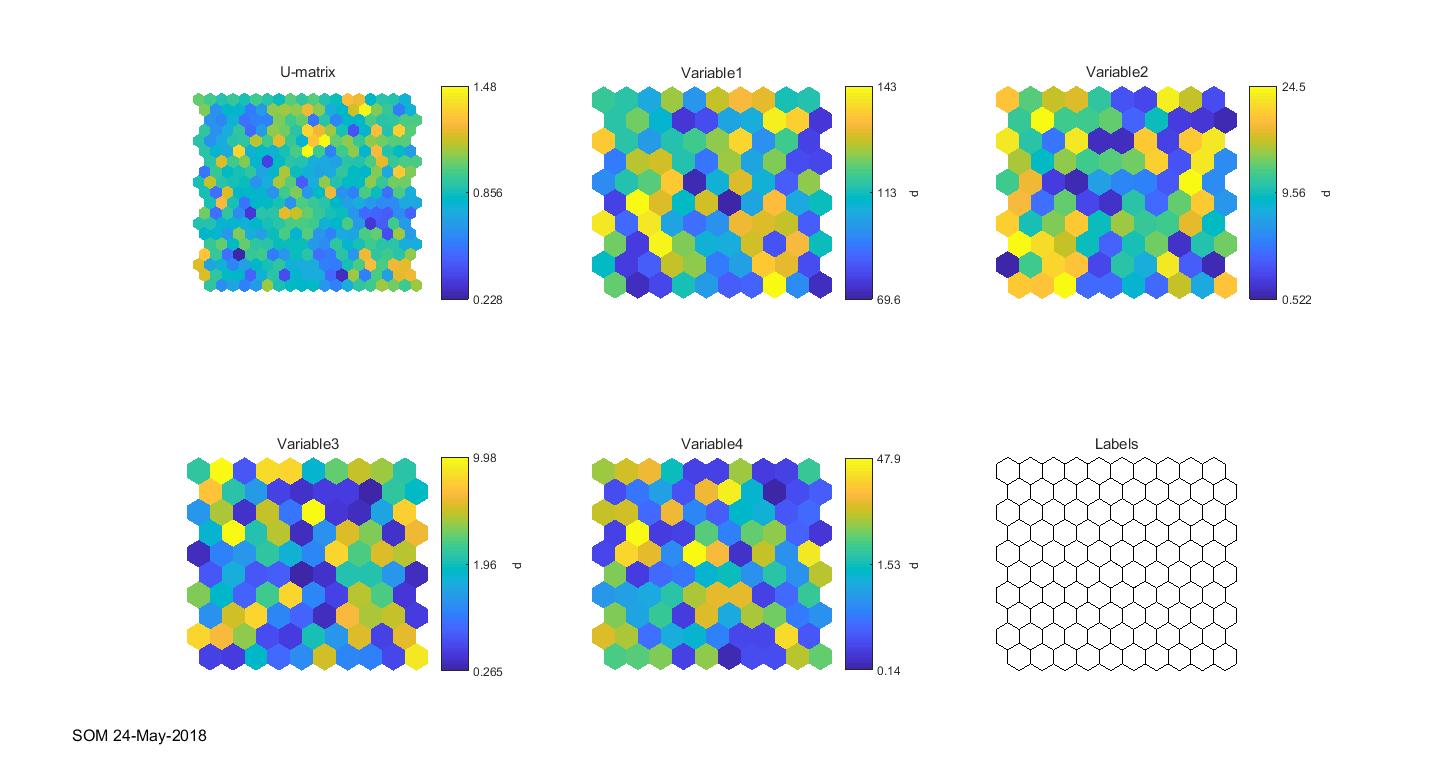
\includegraphics[scale=0.5]{Images/SOM1.png}
	\label{SOM1}
	\caption{Primeiro teste.}
\end{figure*}

\begin{figure*}
	\centering
	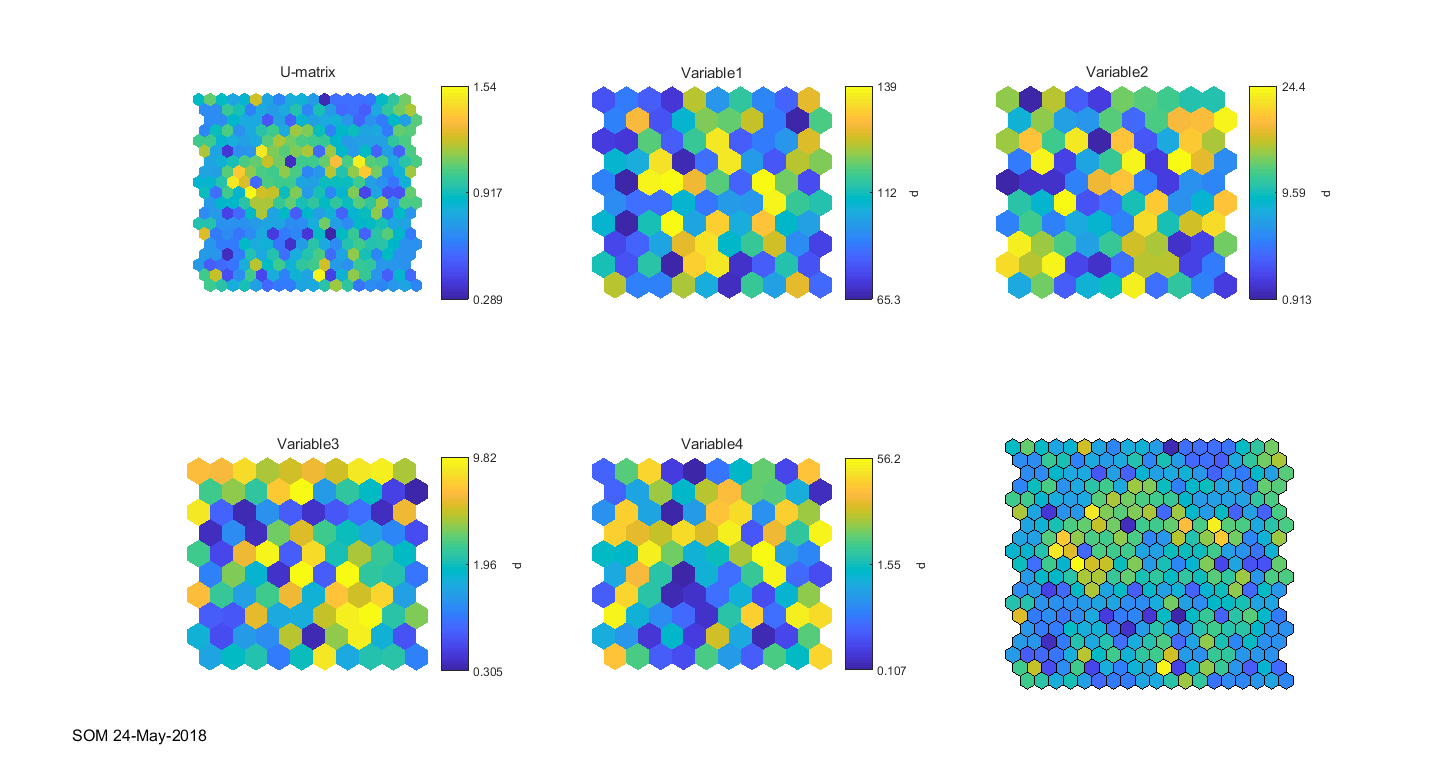
\includegraphics[scale=0.5]{Images/SOM2.png}
	\label{SOM2}
	\caption{Segundo teste.}
\end{figure*}

\begin{figure*}
	\centering
	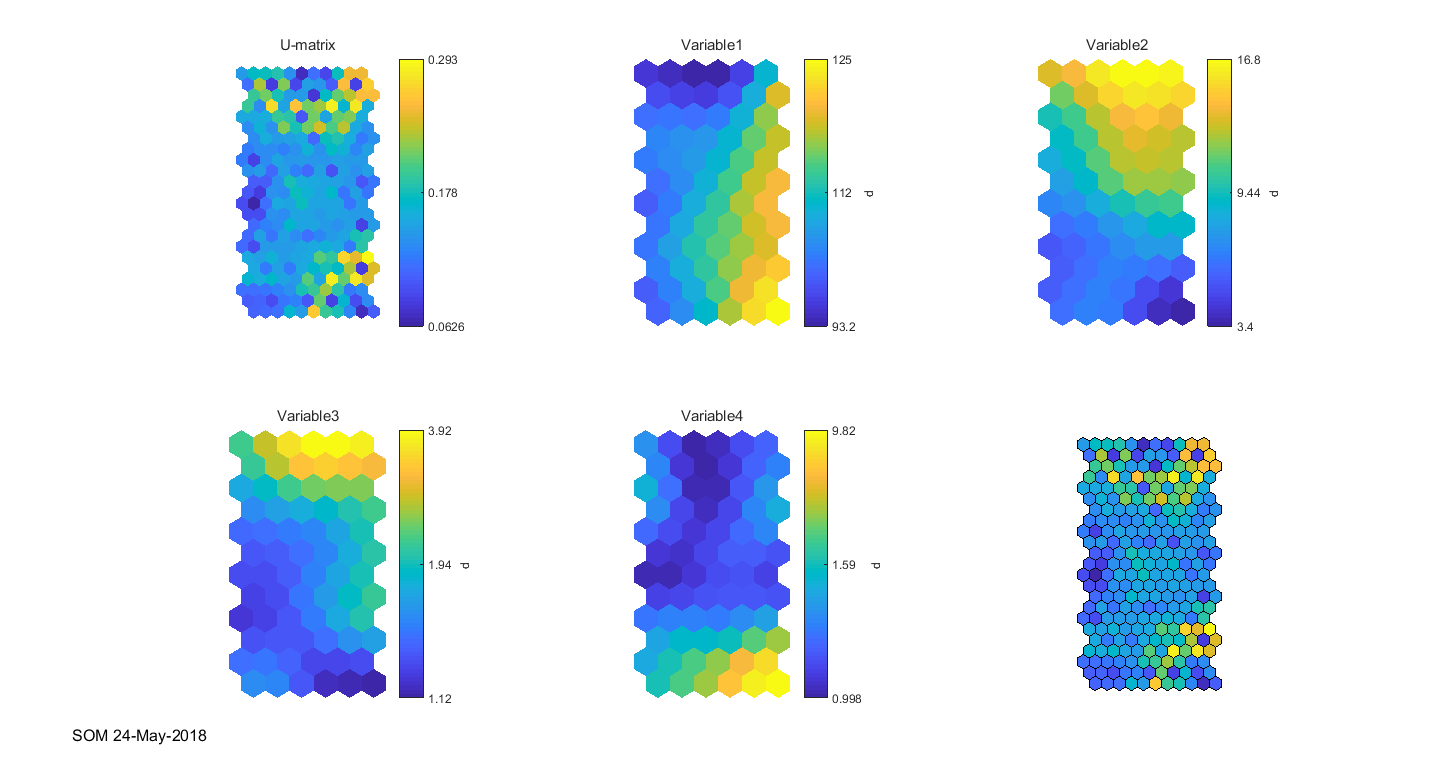
\includegraphics[scale=0.5]{Images/SOM3.png}
	\label{SOM3}
	\caption{Terceiro teste.}
\end{figure*}

\begin{figure*}
	\centering
	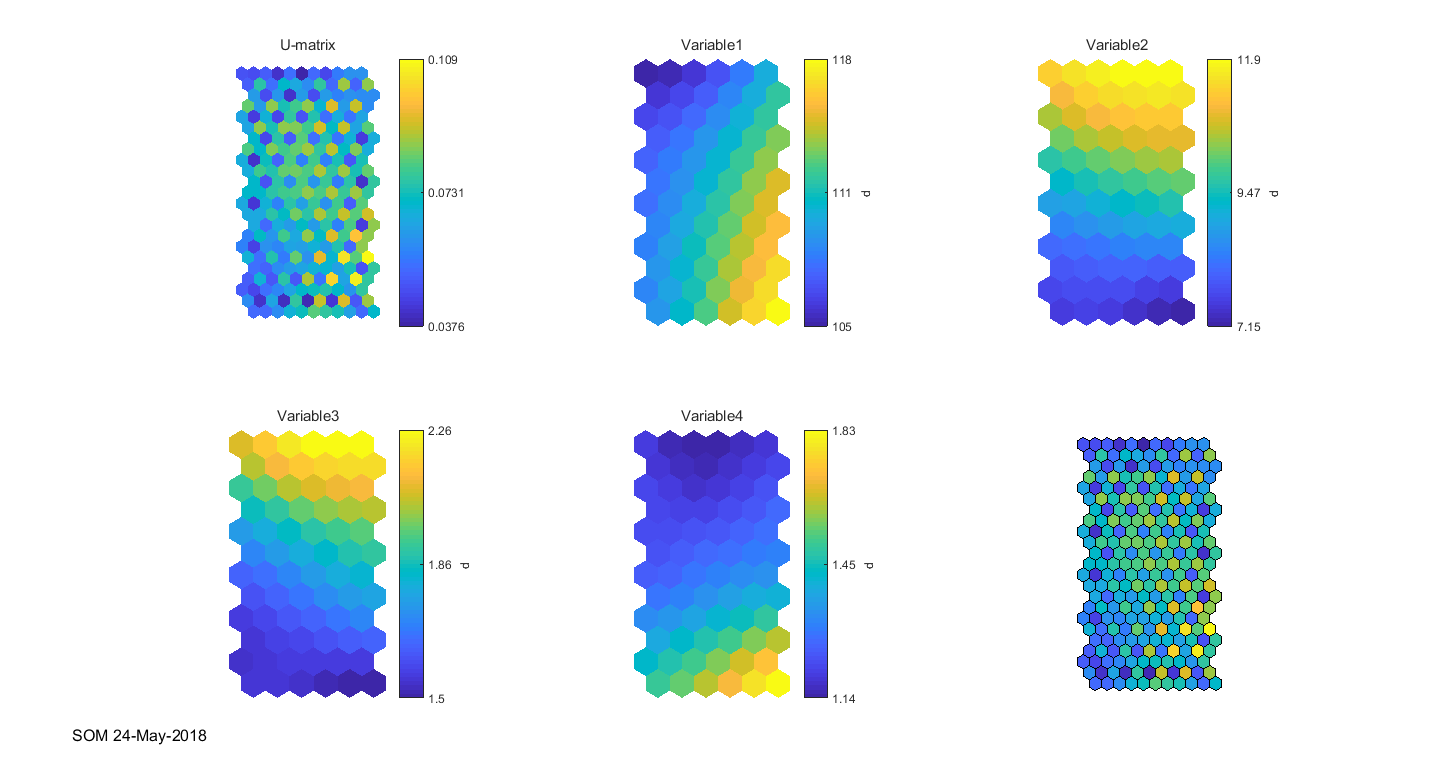
\includegraphics[scale=0.5]{Images/SOM4.png}
	\label{SOM4}
	\caption{Quarto teste.}
\end{figure*}

\section{Conclusões}




% Now we need a bibliography:


\bibliographystyle{apalike}
\bibliography{references}


% Your document ends here!
\end{document}